% (c) 2012 - 2014 Dimitrios Vrettos - d.vrettos@gmail.com
% (c) 2014 Claudio Carboncini - claudio.carboncini@gmail.com
\section{Esercizi}
\subsection{Esercizi dei singoli paragrafi}
\subsubsection*{6.1 - Rappresentazione tabulare}

\begin{esercizio}
\label{ese:6.1}
Dai una rappresentazione tabulare dell'insieme~$A$ dei numeri naturali minori di~6.
\end{esercizio}

\begin{esercizio}
\label{ese:6.2}
Dai una rappresentazione tabulare dei seguenti insiemi
\begin{enumeratea}
 \item delle vocali della parola ``ESERCIZI'';
 \item delle lettere della parola ``RIFLETTERE'';
 \item dei numeri naturali compresi tra~6 e~12, estremi esclusi;
 \item dei numeri dispari compresi tra~10 e~20;
 \item delle lettere dell'alfabeto italiano;
 \item dei numeri naturali minori di~10;
 \item dei multipli di~7;
 \item delle preposizioni con più di due lettere.
\end{enumeratea}
\end{esercizio}

\begin{esercizio}
 \label{ese:6.3}
Indica in rappresentazione tabulare i seguenti insiemi.
\TabPositions{7.5cm}
\begin{enumeratea}
 \item $A=\{x\in\insN\mid x<10\}$\tab\dotfill
 \item $B=\{x\in\insN\mid 2\le x<5\}$\tab\dotfill
 \item $C=\{x\in\insN\mid 5\le x\le~10\}$\tab\dotfill
 \item $D=\{x\in\insN\mid 2x\le~10\}$ \tab\dotfill
 \item $E=\{e\in\insN\mid 5\le e<10\}$\tab\dotfill
 \item $F=\{f\in\insN\mid f\text{ è multiplo di~3 e } f<15\}$\tab\dotfill
 \item $G=\{g\in\insN\mid g\text{ è una cifra del numero }121231\}$\tab\dotfill
 \item $H=\{h\in\insN\mid h=3n+1\text{, con }n\in\insN\}$\tab\dotfill
\end{enumeratea}
\end{esercizio}

\begin{esercizio}
\label{ese:6.4}
Elenca per tabulazione gli elementi di~$A=\{x\mid x\in\insN\text{, }x\text{ è pari, }x\leq10\text{, }x\neq0\}.$
\end{esercizio}

\begin{esercizio}
\label{ese:6.5}
Elenca per tabulazione gli elementi di~$L=\{l\text{ è una lettera della parola MATEMATICA}\}$.
\end{esercizio}

\subsubsection*{6.2 - Rappresentazione caratteristica}

\begin{esercizio}
\label{ese:6.6}
Descrivi mediante la proprietà caratteristica
l'insieme~$D= \{\text{S, T, U, D, I, A, R, E}\}$.
\[D=\{x\mid x\text{ è }\ldots\ldots\ldots\ldots\}\]
\end{esercizio}


\begin{esercizio}
\label{ese:6.7}
Descrivi mediante la proprietà caratteristica l'insieme
\[X=\{\text{1, 2, 3, 4, 5, 6, 7, 8, 9, 10, 11, 12, 13, 14, 15}\}.\]
\[X=\{x\in\insN\mid x\ldots\ldots\ldots\}\]
\end{esercizio}

\begin{esercizio}
\label{ese:6.8}
Descrivi mediante la proprietà caratteristica l'insieme dei numeri primi minori di~$\np{1000}$.
\end{esercizio}

\begin{esercizio}
\label{ese:6.9}
Elenca gli elementi dell'insieme~$I=\{n\in\insN\mid n\text{ è divisore di }12\}$.
\end{esercizio}

\begin{esercizio}
\label{ese:6.10}
Elenca gli elementi dell'insieme~$I=\{n\in\insN\mid n\text{ è multiplo di~3 minore di }20\}$.
\end{esercizio}
\pagebreak
\begin{esercizio}
\label{ese:6.11}
Dato l'insieme~$A=\{\text{2, 4, 8, 16, 32, 64}\}$ quale delle seguenti proprietà caratterizzano i suoi elementi?
\begin{enumeratea}
\item $A=\{n\in\insN\mid n \text{ è numero pari minore di 65}\}$;
\item $A=\{n\in\insN\mid n\text{ è una potenza di 2}\}$;
\item $A=\{n\in\insN\mid n\text{ è una potenza di~2 minore di 65}\}$;
\item $A=\{n\in\insN\mid n=2^{m}\text{, con }m=\text{1, 2, 3, 4, 5, 6}\}$.
\end{enumeratea}
\end{esercizio}

\begin{esercizio}
\label{ese:6.12}
Indica con una proprietà caratteristica l'insieme~$B=\{\text{5, 10, 15, 20, 25, 30, 35, 40, 45, 50}\}$.
\end{esercizio}

\begin{esercizio}
\label{ese:6.13}
Indica con una proprietà caratteristica
l'insieme~$B=\{\text{4, 9, 16, 25, 36, 49, 64, 81}\}$.
\end{esercizio}

\begin{esercizio}
\label{ese:6.14}
Quale delle seguenti frasi indica la proprietà caratteristica
di~$A=\{\text{0, 4, 8, 12, 16, 20, }\ldots\}$
\begin{center}
\boxA\quad I multipli di~2; \quad\boxB\quad i numeri pari; \quad\boxC\quad i multipli di~4; \quad\boxD\quad i divisori di~20.
\end{center}
\end{esercizio}

\begin{esercizio}
\label{ese:6.15}
Rappresenta in forma caratteristica i seguenti insiemi.
\begin{enumeratea}
\item $A=\{\text{5, 6, 7, 8, 9, 10}\}$;
\item $B=\{\text{0, 1, 2, 3, 4, 5, \ldots, 98, 99, 100}\}$;
\item$ C=\{\text{0, 3, 6, 9, 12, 15, 18, 21, 24, 27, 30}\}$.
\end{enumeratea}
\end{esercizio}

\begin{esercizio}
\label{ese:6.16}
Quale delle seguenti è una rappresentazione per caratteristica
dell'insieme
\[D = \{\text{0, 3, 6, 9, 12, 15, 18}\}.\]
\begin{enumeratea}
\item $D=\{x\in\insN\mid x\le~18\}$;
\item $D=\{x\in\insN\mid x\text{ è multiplo di~3 e }x<20\}$;%
\item $D=\{x\in\insN\mid x=3x\}$;
\item $D=\{x\in\insN\mid x=3\}$.
\end{enumeratea}
\end{esercizio}

\begin{esercizio}
\label{ese:6.17}
Rappresenta i seguenti insiemi con la proprietà caratteristica.
\begin{enumeratea}
 \item $A=\{\text{gennaio, maggio, giugno, luglio, agosto}\}$;
 \item $B=\{\text{Gorizia, Pordenone, Trieste, Udine}\}$;
 \item $C=\{\text{sabato, domenica}\}$;
 \item $D=\{\text{10, 20, 30, 40, 50}\}$;
 \item $E=\{\text{Puglia, Piemonte}\}$.
 \end{enumeratea}
\end{esercizio}

\begin{esercizio}
Individua una proprietà caratteristica dei seguenti insiemi numerici.
\label{ese:6.18}
\begin{enumeratea}
\spazielenx
 \item $A=\{\text{4, 9, 16, 25, \ldots}\}$;
 \item $B=\bigg\{\dfrac{1}{4}\text{, }\dfrac{1}{9}\text{, }\dfrac{1}{16}\text{, }\dfrac{1}{25}\text{, }\ldots\bigg\}$;
 \item $C=\bigg\{2\text{, }\dfrac{3}{2}\text{, }\dfrac{4}{3}\text{, }\dfrac{5}{4}\text{, }\dfrac{6}{5}\text{, }\ldots\bigg\}$;
 \item $D=\bigg\{\dfrac{1}{5}\text{, }\dfrac{1}{10}\text{, }\dfrac{1}{15}\text{, }\dfrac{1}{20}\text{, }\ldots\bigg\}$;
 \item $E=\bigg\{\dfrac{1}{4}\text{, }\dfrac{2}{9}\text{, }\dfrac{3}{16}\text{, }\dfrac{4}{25}\text{, }\dfrac{5}{36}\text{, }\ldots\bigg\}$;
 \item $F=\{+1\text{, }-2\text{, }+4\text{, }-8\text{, }+16\text{, }-32\text{, }+64\text{, }\ldots\}$.
 \end{enumeratea}
\end{esercizio}

\begin{esercizio}
\label{ese:6.19}
Elenca gli elementi dei seguenti insiemi.
\begin{enumeratea}
\item $A=\{x\in\insZ\mid -3\le x<2\}$;
\item $B=\{x\in\insN\mid -4\le x\le~1\text{ o }5<x\le~7\}$.
\end{enumeratea}
\end{esercizio}

\begin{esercizio}
\label{ese:6.20}
Rappresenta in forma caratteristica i seguenti insiemi.
\begin{enumeratea}
\item $A=\{\text{0, 2, 4, 6, 8, 10}\}$;
\item $B=\{\text{1, 4, 9, 16, 25, 36, 49, \ldots}\}$;
\item $C=\{\text{3, 4, 5, 6, 7}\}$;
\item $D=\{-5\text{, }-4\text{, }-3\text{, }-2\text{, }-1\text{, }0\text{, }+1\text{, }+2\text{, }+3\text{, }+4\text{, }+5\}$;
\item $E=\{\text{0, 10, 20, 30, 40, 50, 60, 70, 80, 90, 100}\}$;
\item $F=\{\text{1, 4, 9, 16, 25, 36, 49, 64, 81, 100}\}$.
\end{enumeratea}
\end{esercizio}

\subsubsection*{6.3 - Rappresentazione grafica (Diagramma di Eulero-Venn)}

\begin{esercizio}
\label{ese:6.21}
Rappresenta con un diagramma di Eulero-Venn l'insieme:
\begin{enumeratea}
\item dei multipli di~3 compresi tra~10 e~30, estremi inclusi;
\item delle note musicali;
\item dei numeri primi minori di~20;
\item delle consonanti della parola ``MATEMATICA'';
\item delle province della Toscana.
\end{enumeratea}
\end{esercizio}

\begin{esercizio}
\label{ese:6.22}
In base agli insiemi~$A$ e~$B$ rappresentati dai diagrammi di Eulero-Venn, stabilisci quali affermazioni sono vere.
\begin{multicols}{2}
\TabPositions{2.5cm}
\begin{enumeratea}
\item $5\notin B$\tab\boxV\quad\boxF
\item $A=\emptyset $\tab\boxV\quad\boxF
\item $3+2\in A$\tab\boxV\quad\boxF
\item $B\neq \emptyset $\tab\boxV\quad\boxF
\item $6\in B$\tab\boxV\quad\boxF
\item $9\notin A$\tab\boxV\quad\boxF
\end{enumeratea}
\columnbreak
% (c) 2012 Dimitrios Vrettos - d.vrettos@gmail.com
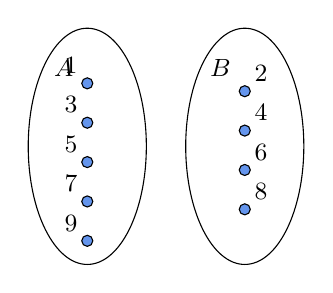
\begin{tikzpicture}[x=.5cm,y=1cm,font=\small]
    \draw (0,0)circle (1.5) (0,1) node[ left=1.5] {$A$};
    \begin{scope}[fill=CornflowerBlue, draw=black]
\filldraw (0,.8) circle (2pt) node[above left] {1};
\filldraw (0,.3) circle (2pt) node[above left] {3};
\filldraw (0,-.2) circle (2pt) node[above left] {5};
\filldraw (0,-.7) circle (2pt) node[above left] {7};
\filldraw (0,-1.2) circle (2pt) node[above left] {9};
\begin{scope}[xshift=2cm]
    \draw (0,0)circle (1.5) (0,1) node[ left=1.5] {$B$};
\filldraw (0,.7) circle (2pt) node[above right] {2};
\filldraw (0,.2) circle (2pt) node[above right] {4};
\filldraw (0,-.3) circle (2pt) node[above right] {6};
\filldraw (0,-.8) circle (2pt) node[above right] {8};
\end{scope}
\end{scope}
\end{tikzpicture}

\end{multicols}
\end{esercizio}

\subsection{Esercizi riepilogativi}

\begin{esercizio}
Scrivi i primi dieci elementi dei seguenti insiemi.
\begin{enumeratea}
\spazielenx
\item $A=\{x\mid x=2n\text{, }n\in\insN\}$;
\item $B=\{x\mid x=n^{2}\text{, }n\in\insN\}$;
\item $C=\{x\mid x=2n^{2}\text{, }n\in\insN\}$;
\item $D=\{x\mid x=2n+2\text{, }n\in\insN\}$;
\item $E=\{x\mid x=n^{2}-n\text{, }n\in\insN\}$;
\item $E=\{x\mid x=\dfrac{n+1}{n-1}\text{, }x\in\insZ\text{, }n\in\insN\}$.
\end{enumeratea}
\end{esercizio}

\begin{esercizio}
Rappresenta i seguenti insiemi con rappresentazione tabulare, caratteristica e grafica.
\begin{enumeratea}
\item Insieme~$A$ dei divisori di~30;
\item insieme~$B$ dei numeri pari minori o uguali a~10;
\item l'insieme~$C$ delle province della Puglia;
\item l'insieme~$D$ delle lettere della parola ``COCCO''.
\end{enumeratea}
\end{esercizio}

\begin{esercizio}
Rappresenta nel modo che ritieni più opportuno gli insiemi i cui elementi sono:
\begin{enumeratea}
\item i numeri naturali multipli di~5 compresi tra~10 e~$\np{10000}$;
\item i colori dell'arcobaleno;
\item i numeri razionali maggiori o uguali a~$2/7$;
\item i punti di una superficie~$S$;
\item le lettere di cui è composto il tuo nome.
\end{enumeratea}
\end{esercizio}

\begin{esercizio}
Rappresenta con una modalità a tua scelta l'insieme dei numeri interi multipli di~5 maggiori di~10 e minori di~100 che non
sono dispari.
\end{esercizio}

\begin{esercizio}
Dati gli insiemi:~$X=\{\text{8, 9, 10}\}$, $Y=\{\text{0, 8, 9, 10}\}$, $H=\{\text{10, 9, 8}\}$,
$W=\{w\in\insN\mid 8\le w\le 10\}$, $Z=\{z\in\insN\mid 8<z\le10\}$ e~$J=\{j\in\insN\mid 7<j<11\}$,
individua le uguaglianze corrette.
\begin{multicols}{3}
\begin{enumeratea}
\item $X = Y$;
\item $X= H$;
\item $W = H$;
\item $X = Z$;
\item $\card Z=2$;
\item $X = J$.
\end{enumeratea}
\end{multicols}
\end{esercizio}

\begin{esercizio}
Dati gli insiemi:
$A=\{$g, a, t, o$\}$, $B=\{$o, g, t, a$\}$, $C=\{c\mid c$ è una lettera della parola ``gatto''$\}$,
$D=\{$g, t$\}$, $E=\{$gatto$\}$, $F=\{f\mid f$ è una consonante della parola ``gatto''$\}$,
segna con una crocetta le uguaglianze corrette:
\begin{multicols}{4}
\begin{enumeratea}
 \item $A = B$;
 \item $A = D$;
 \item $A = C$;
 \item $E = A$;
 \item $C = E$;
 \item $D = F$;
 \item $C = D$:
 \item $D = E$.
 \columnbreak
 \item $\card C=5$;
 \item $\card E=5$;
\end{enumeratea}
\end{multicols}
\end{esercizio}

\begin{esercizio}
Per ciascuno dei seguenti insiemi indica alcuni elementi.
\TabPositions{6cm}
\begin{enumeratea}
\item $X=\{x\in\insN\mid x-1\text{ è pari }\}$\dotfill
\item $Y=\{y\in\insN\mid y=3n\text{, con } n\in\insN\}$\dotfill
\item $Z=\{z\in\insN\mid z=3n\text{ e } z\text{ non è divisibile per~2, }n\in\insN\}$\dotfill
\item $W=\{w\in\insN\mid w<0\}$\dotfill
\end{enumeratea}
\end{esercizio}

\begin{esercizio}
Quali delle seguenti scritture sono vere?
\begin{enumeratea}
\TabPositions{7cm}
\item $5\in \{\text{10, 8, 6, 4, 2}\}$\tab\boxV\quad\boxF
\item $15\in \{n\in\insN\mid n\ge~10\}$\tab\boxV\quad\boxF
\item $7\in \{n\in\insN\mid n+5<10\}$\tab\boxV\quad\boxF
\item $l\notin\{x\mid x\text{ è una lettera della parola ``scuola''}\}$\tab\boxV\quad\boxF
\end{enumeratea}
\end{esercizio}

\begin{esercizio}
Quali dei seguenti insiemi sono uguali?
 \begin{enumeratea}
 \item $A=\{1+3\text{, }5-2\text{, }1+1\text{, }9-8\text{, }1-1\}$;
\item $B=\{n\in\insN\mid n<5\}$;
\item $C=\{6-4\text{, }6+4\text{, }6-6\}$.
 \end{enumeratea}
\end{esercizio}
\pagebreak
\begin{esercizio}
Quali dei seguenti insiemi sono uguali?
\begin{multicols}{2}
\begin{enumeratea}
\item $A=\{x\in\insN\mid 3\le x\le~12\}$;
\item $B=\{x\in\insN\mid x=3\cdot n\text{, con } 1\le n\le~4\}$;
\item $A=\{x\in\insN\mid 2<x<13\}$;
\item $B=\{x\in\insN\mid x=3^{n}\text{, con }n=\text{1, 2, 3, 4}\}$.
\end{enumeratea}
\end{multicols}
\end{esercizio}
